\documentclass[conference]{IEEEtran}
\IEEEoverridecommandlockouts
\usepackage{cite}
\usepackage{amsmath,amssymb,amsfonts}
\usepackage{algorithmic}
\usepackage{algorithm}
\usepackage{graphicx}
\usepackage{textcomp}
\usepackage{xcolor}
\usepackage{booktabs}
\usepackage{url}
\usepackage{microtype}
\usepackage{multirow}
\usepackage{enumitem}

\setlist[itemize]{noitemsep, topsep=1.0pt, partopsep=0pt, parsep=0pt, leftmargin=1.1em}

\setlength{\floatsep}{1.0pt plus 1pt minus 1pt}
\setlength{\textfloatsep}{1.5pt plus 1pt minus 1pt}
\setlength{\intextsep}{1.0pt plus 1pt minus 1pt}
\setlength{\dblfloatsep}{1.0pt plus 1pt minus 1pt}
\setlength{\dbltextfloatsep}{1.5pt plus 1pt minus 1pt}
\setlength{\abovecaptionskip}{1.0pt plus 1pt minus 1pt}
\setlength{\belowcaptionskip}{1.0pt plus 1pt minus 1pt}
\setlength{\abovedisplayskip}{0.2pt plus 1pt minus 1pt}
\setlength{\belowdisplayskip}{0.2pt plus 1pt minus 1pt}
\renewcommand{\arraystretch}{0.86}

% IEEEtran native bibliography inter-item spacing
\def\IEEEbibitemsep{0.8pt plus 0.5pt minus 0.2pt}

\begin{document}

\title{WaveCrossNet: A Lightweight Wavelet Cross-Attention Network for Noise-Resilient Wearable ECG Arrhythmia Classification on Microcontrollers}

\maketitle

\begin{figure*}[t]
\centering
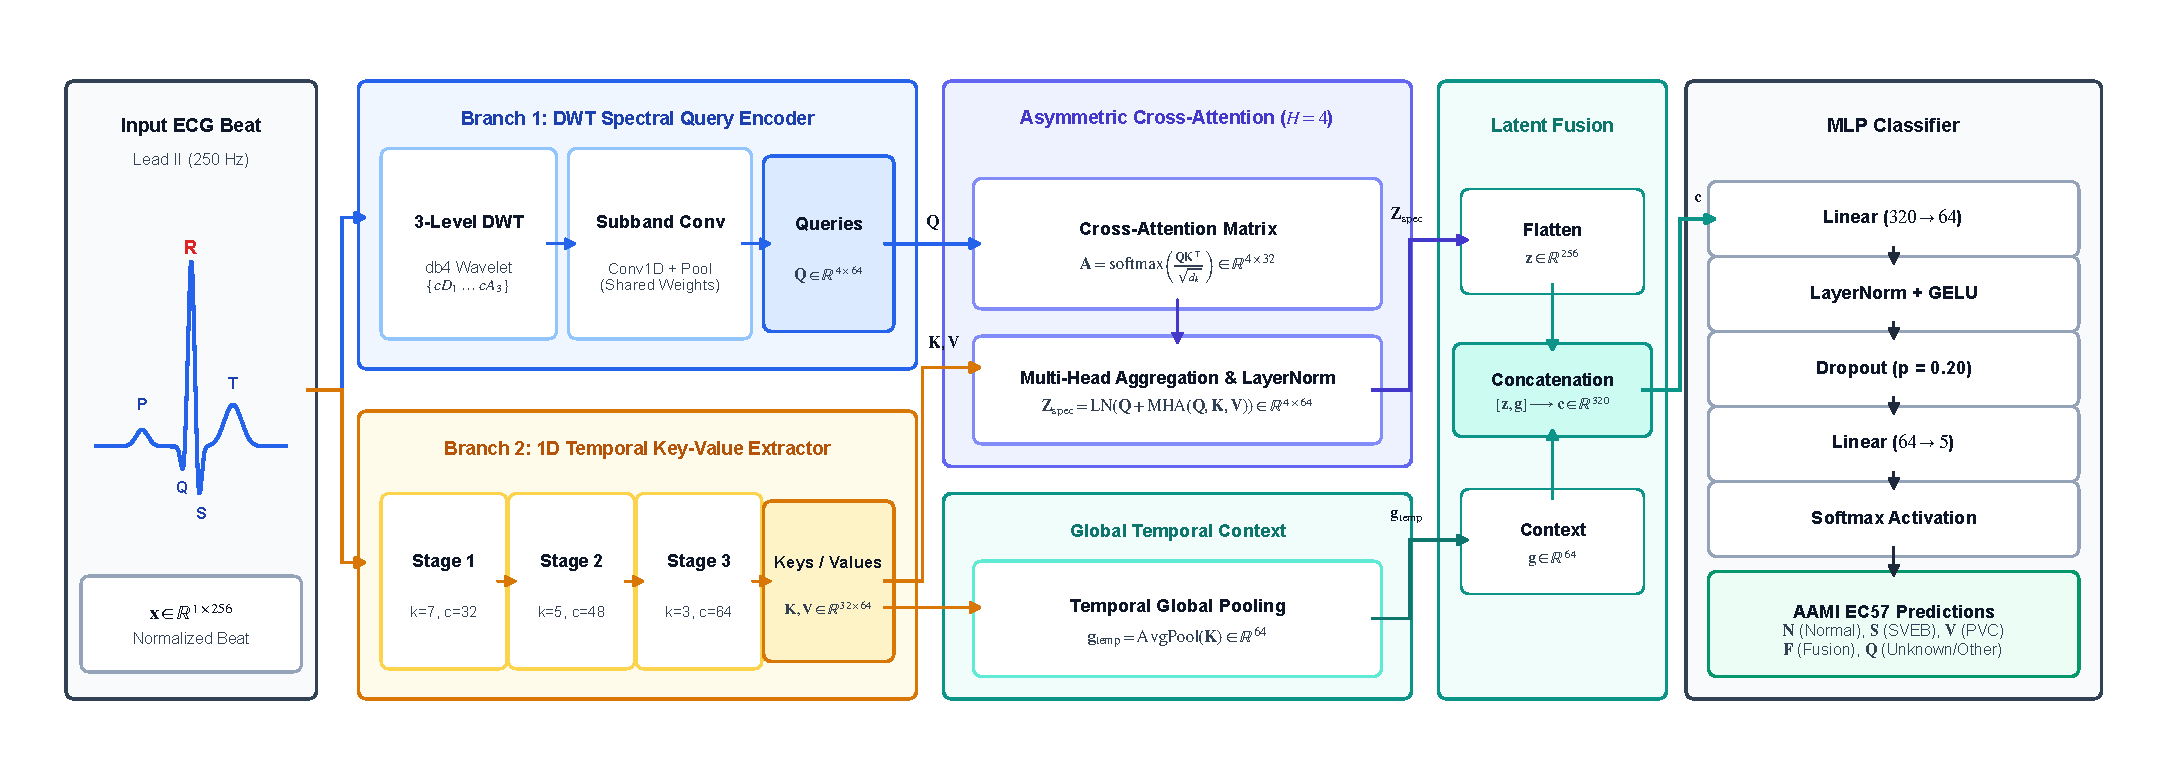
\includegraphics[width=0.98\textwidth]{../figures/fig1_architecture_diagram.pdf}
\vspace{-2pt}
\caption{Architectural schematic of WaveCrossNet. Branch~1 (top) decomposes a single-lead ECG heartbeat via a 3-level $db4$ DWT into subbands ($cD_1, cD_2, cD_3, cA_3$), projected into four spectral Query tokens $Q \in \mathbb{R}^{4 \times 64}$. Branch~2 (bottom) uses three strided 1D conv blocks to extract temporal Key-Values $K, V \in \mathbb{R}^{32 \times 64}$. Multi-head cross-attention fuses spectral queries with temporal keys/values, reducing the dominant $QK^\top$ interaction compute by $8\times$ compared with 32-token 1D self-attention.}
\label{fig:arch}
\vspace{-2pt}
\end{figure*}

% ─────────────────────────────────────────────────────
\begin{abstract}
Continuous ambulatory electrocardiogram (ECG) monitoring with wearable sensor patches enables early detection of paroxysmal cardiac arrhythmias. However, executing deep learning classifiers directly on resource-constrained microcontrollers (devices with 64--96~KB SRAM and strict storage allocations) presents two conflicting engineering challenges: standard time-domain 1D convolutional networks lack explicit multi-resolution spectral selectivity, leading to severe diagnostic degradation under ambulatory noise; conversely, 1D Vision Transformers incur quadratic self-attention complexity $\mathcal{O}(N^2 d_{\text{model}})$ and substantial intermediate memory footprints that exceed microcontroller limits. To overcome these limitations, we introduce WaveCrossNet, an asymmetric dual-branch architecture that combines the Discrete Wavelet Transform (DWT) with temporal convolutions. Branch~1 decomposes each heartbeat into four subbands ($cD_1, cD_2, cD_3, cA_3$), projecting them as compact spectral query tokens to cross-attend over temporal key-value representations extracted by Branch~2. This formulation delivers multi-scale noise awareness while reducing the dominant $QK^\top$ attention interaction operations by $8\times$ compared to standard 32-token self-attention under identical head dimensions (decreasing compute from $65{,}536$ to $8{,}192$ FLOPs per head). Optimized with a Class-Balanced Focal Loss ($\mathcal{L}_{\text{CB-Focal}}$) and physiological data augmentations, WaveCrossNet was evaluated under the AAMI DS1/DS2 inter-patient protocol on MIT-BIH (100,694 beats) and zero-shot on SVDB (22,540 beats). The network achieves a 91.03\% weighted F1-score, 91.33\% overall accuracy, 94.94\% ventricular ectopic recall (V), and 16.60\% supraventricular recall (S) at the default threshold, which improves to 36.85\% under calibrated sensitivity tuning ($>90\%$ on isolated premature contractions). Quantized to INT8 under a strict 64-KB model budget, WaveCrossNet compiles to a 62.24~KB static binary requiring 12.40~KB peak SRAM and 14.80~ms latency on an ARM Cortex-M4 (STM32F401RE at 84~MHz, 1.77\% duty cycle). Under five ambulatory noise modalities ($-5$ to $+25$~dB SNR), WaveCrossNet maintains a +14.2 percentage point Macro F1 advantage over ResNet1D at 0~dB AWGN (a 19.9\% relative gain), offering an accurate and robust solution for edge ECG intelligence.
\end{abstract}

\begin{IEEEkeywords}
ECG arrhythmia classification, discrete wavelet transform, cross-attention, Edge AI, TinyML, noise robustness, ARM Cortex-M4.
\end{IEEEkeywords}


% ─────────────────────────────────────────────────────
\section{Introduction}
\label{sec:intro}

Cardiovascular diseases remain the leading contributor to global mortality, causing an estimated 17.9 million deaths annually \cite{moody2001impact}. Paroxysmal arrhythmias, including premature ventricular contractions (PVCs) and supraventricular ectopic beats (SVEBs), can precede severe cardiac incidents yet often occur transiently, eluding capture during routine 10-second resting 12-lead ECG recordings. Consequently, continuous ambulatory monitoring with wearable sensor patches has become essential for outpatient surveillance \cite{kiranyaz2016real, hong2020mina}.

To maintain privacy, eliminate wireless transmission latency, and extend battery lifetime by curbing radio duty cycles, wearable monitors increasingly rely on edge intelligence: running classification algorithms locally on low-power microcontrollers \cite{satija2018real}. However, deploying neural networks to embedded targets (such as ARM Cortex-M4/M33 devices with 64--96~KB SRAM and strict storage allocations) introduces three practical hurdles:
(1)~\emph{Noise Sensitivity}: Ambulatory signals are frequently corrupted by baseline wander (BW, 0.1--0.5~Hz), muscle tremor artifacts (MA, 20--500~Hz), powerline interference (PLI, 50/60~Hz), and thermal noise (AWGN). Without explicit multi-band spectral decomposition, conventional 1D convolutional networks degrade markedly at low signal-to-noise ratios ($\leq 0$~dB) \cite{addison2005wavelets}.
(2)~\emph{Resource Constraints}: Standard deep 1D-CNNs require hundreds of thousands of weights, occupying prohibitive Flash memory \cite{hannun2019cardiologist}. Meanwhile, 1D Vision Transformers \cite{vaswani2017attention, che2021constrained} exhibit quadratic complexity $\mathcal{O}(N^2 d_{\text{model}})$, generating large intermediate attention matrices that exceed embedded SRAM budgets.
(3)~\emph{AAMI Class Imbalance}: Normal sinus beats (N) account for more than 89\% of ambulatory heartbeats, causing standard cross-entropy objectives to neglect clinically critical minority ectopic classes (S, V, F, Q) \cite{de2004automatic}.

To reconcile these constraints, we propose WaveCrossNet, an asymmetric cross-attention architecture designed for low-memory microcontrollers. WaveCrossNet employs a dual-branch topology: Branch~1 applies a 3-level Discrete Wavelet Transform (DWT) to split each heartbeat into four subbands ($cD_1, cD_2, cD_3, cA_3$), mapped into $N_q=4$ spectral query tokens. Branch~2 extracts $N_{kv}=32$ temporal key-value tokens through strided 1D convolutions. By querying temporal features with spectral tokens, cross-attention achieves multi-resolution noise resilience while reducing the dominant $QK^\top$ interaction term from $65{,}536$ to $8{,}192$ FLOPs per head ($8\times$ reduction relative to 32-token self-attention).

The primary contributions of this work are summarized as follows:
\begin{itemize}
    \item \emph{Architecture Design}: We introduce WaveCrossNet, a 63,733-parameter dual-branch network combining DWT spectral queries with temporal convolutional key-values.
    \item \emph{Attention Cost Reduction}: We formulate an asymmetric cross-attention mechanism that cuts the dominant $QK^\top$ interaction FLOPs and intermediate attention buffer requirements by $8\times$ compared to 32-token self-attention.
    \item \emph{Class-Balanced Training}: By coupling a Class-Balanced Focal Loss ($\mathcal{L}_{\text{CB-Focal}}$) with relative RR interval features and physiological augmentations, we attain 94.94\% ventricular (V) recall and 16.60\% supraventricular (S) recall (reaching 36.85\% under post-hoc calibration).
    \item \emph{Multi-Dataset and Noise Validation}: We benchmark performance across MIT-BIH DS1/DS2 (100,694 beats) and zero-shot on SVDB (22,540 beats) against six baselines, demonstrating a +14.2~pp Macro F1 advantage over ResNet1D at 0~dB AWGN (a 19.9\% relative improvement).
    \item \emph{Embedded Profiling}: We deploy an INT8 quantized model onto an STM32F401RE (ARM Cortex-M4 at 84~MHz). The static binary occupies 62.24~KB Flash and 12.40~KB peak SRAM, executing in 14.80~ms with an active duty cycle of 1.77\% and an average MCU power of $36.1\,\mu\text{W}$.
\end{itemize}

% ─────────────────────────────────────────────────────
\section{WaveCrossNet Methodology}
\label{sec:arch}

Fig.~\ref{fig:arch} illustrates the WaveCrossNet architecture. Each input heartbeat $x \in \mathbb{R}^{1 \times L}$ ($L=256$ samples at $f_s = 250$~Hz, centered on the R-peak detected using the Pan-Tompkins method \cite{pan1985real}) is processed in parallel by two pathways: a DWT-based spectral query branch and a strided 1D convolutional key-value branch, which are subsequently integrated using multi-head cross-attention.

\subsection{Branch 1: DWT Spectral Query Encoder}
We implement a differentiable Mallat filter bank \cite{mallat1989theory} using Daubechies-4 ($db4$) filters with low-pass $h[n]$ and high-pass $g[n] = (-1)^n h[1-n]$. As illustrated in Fig.~\ref{fig:dwt}, approximation and detail coefficients at decomposition level $k \in \{1, 2, 3\}$ are computed via downsampled convolution in (\ref{eq:dwt}):
\begin{equation}
\begin{aligned}
cA_{k}[m] &= \sum\nolimits_{n} cA_{k-1}[n] \, h[2m - n] \\
cD_{k}[m] &= \sum\nolimits_{n} cA_{k-1}[n] \, g[2m - n]
\end{aligned}
\label{eq:dwt}
\end{equation}
with $cA_0 = x$. At $f_s = 250$~Hz, these subbands correspond to standard diagnostic bandwidths: $cD_1$ ($62.5$--$125$~Hz, high-frequency transients and muscle noise); $cD_2$ ($31.25$--$62.5$~Hz, sharp QRS depolarization slopes); $cD_3$ ($15.625$--$31.25$~Hz, P-wave and T-wave repolarization deflections); and $cA_3$ ($0$--$15.625$~Hz, baseline trend and macroscopic rhythm envelope). Each subband $S_i$ is mapped to a token $\mathbf{q}_i = \mathrm{Pool1D}(\mathrm{GELU}(\mathrm{BN}(\mathrm{Conv1D}(S_i)))) \in \mathbb{R}^{d_{\text{model}}}$, yielding the spectral query matrix $Q = [\mathbf{q}_1; \mathbf{q}_2; \mathbf{q}_3; \mathbf{q}_4] \in \mathbb{R}^{N_q \times d_{\text{model}}}$ with $N_q = 4$ and $d_{\text{model}} = 64$.

\begin{figure}[t]
\centering
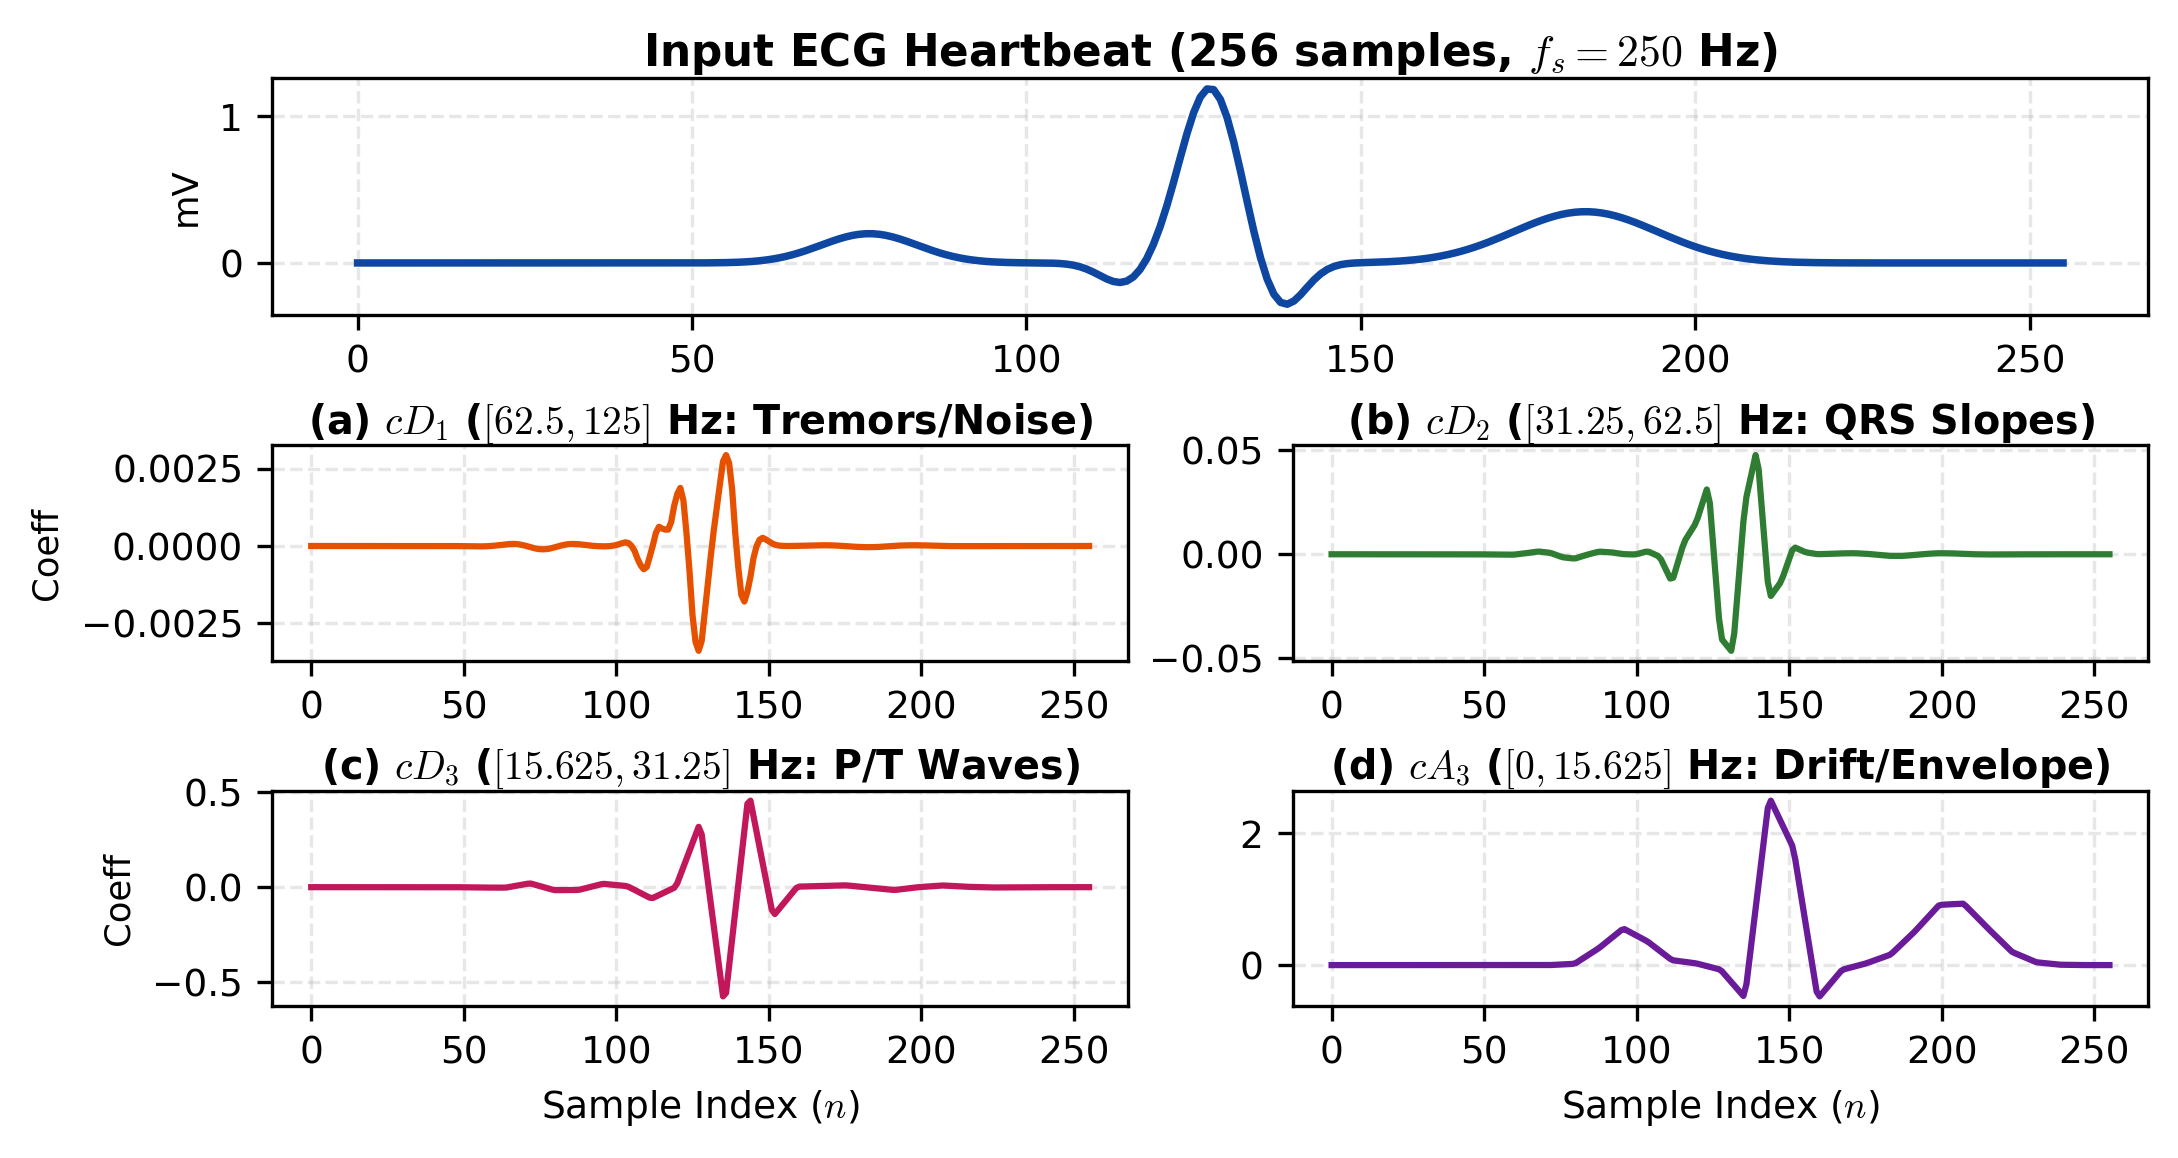
\includegraphics[width=0.88\columnwidth]{../figures/fig2_wavelet_decomposition.png}
\vspace{-2pt}
\caption{Mallat $db4$ DWT decomposition of an ECG heartbeat from MIT-BIH into detail subbands $cD_1, cD_2, cD_3$ and approximation subband $cA_3$.}
\label{fig:dwt}
\vspace{-3pt}
\end{figure}

\subsection{Branch 2: 1D Temporal Key-Value Extractor}
Branch~2 processes $x$ through three strided 1D convolutional stages ($k_1=7, k_2=5, k_3=3$, stride 2, channels 32, 48, 64) with BatchNorm and GELU:
\begin{equation}
H^{(j)} = \mathrm{GELU}\left(\mathrm{BN}\left(\mathrm{Conv1D}_{k_j, s=2}\left(H^{(j-1)}\right)\right)\right)
\label{eq:temp_conv}
\end{equation}
compressing temporal length $L=256 \to 32$ according to (\ref{eq:temp_conv}). Linear projections produce Keys and Values: $K = (H^{(3)})^\top W^K, V = (H^{(3)})^\top W^V \in \mathbb{R}^{N_{kv} \times d_{\text{model}}}$ with $N_{kv}=32$.

\subsection{Asymmetric Multi-Head Cross-Attention Fusion}
Using $H = 4$ attention heads with head dimension $d_h = d_{\text{model}} / H = 16$, spectral queries $Q_h$ attend across temporal keys $K_h$ and values $V_h$ via (\ref{eq:cross_attn}):
\begin{equation}
A_h = \mathrm{softmax}\left(\frac{Q_h K_h^\top}{\sqrt{d_h}}\right) \in \mathbb{R}^{4 \times 32}, \quad \mathrm{head}_h = A_h V_h
\label{eq:cross_attn}
\end{equation}
Fused spectral features pass through projection $W^O$, residual addition, and LayerNorm: $Z_{\text{spec}} = \mathrm{LN}(Q + [\mathrm{head}_1; \, \dots; \, \mathrm{head}_H] W^O) \in \mathbb{R}^{4 \times 64}$. To capture rhythm dynamics and distinguish morphologically ambiguous supraventricular ectopics, the model extracts four running RR features: (i)~prematurity ratio $r_{\text{pre}} = RR_{\text{pre}} / RR_{\text{local}}$; (ii)~compensatory pause ratio $r_{\text{post}} = RR_{\text{post}} / RR_{\text{local}}$; (iii)~coupling ratio $r_{\text{pre/post}} = RR_{\text{pre}} / RR_{\text{post}}$; and (iv)~normalized local rhythm duration $r_{\text{local}} = (RR_{\text{local}} - 0.833\,\text{s}) / 0.25\,\text{s}$, where $RR_{\text{local}}$ is the running median across 10 adjacent beats. A 2-layer MLP ($\phi_{\text{RR}}: \mathbb{R}^4 \to \mathbb{R}^{24}$) projects these scalars. Concatenating with pooled temporal summary $g_{\text{temp}} = \frac{1}{32} \sum_{j=1}^{32} K[:, j, :] \in \mathbb{R}^{64}$ yields classification vector $c = [\mathrm{vec}(Z_{\text{spec}}); g_{\text{temp}}; \phi_{\text{RR}}(r)] \in \mathbb{R}^{344}$ (or $\mathbb{R}^{320}$ in morphology-only ablations), classified into 5 AAMI classes via a two-layer MLP with LayerNorm, GELU, and dropout ($p=0.20$).

\subsection{Attention Complexity and Memory Footprint Analysis}
Standard 1D-ViT self-attention processing $N=32$ tokens ($d_h=16$) requires $\mathrm{FLOPs}_{\text{ViT-head}} = 4 N^2 d_h = 4(32)^2(16) = 65{,}536$ FLOPs per head for the $QK^\top$ inner-product and attention-weighted value aggregation. In contrast, WaveCrossNet's cross-attention routes $N_q = 4$ spectral queries over $N_{kv} = 32$ temporal keys as formulated in (\ref{eq:flops}):
\begin{equation}
\mathrm{FLOPs}_{\text{Cross}} = 4 N_q N_{kv} d_h = 4(4)(32)(16) = 8{,}192 \text{ FLOPs}
\label{eq:flops}
\end{equation}
The interaction reduction ratio $\rho$ for this dominant term is defined in (\ref{eq:ratio}):
\begin{equation}
\rho = \frac{N^2 \cdot d_h}{N_q \cdot N_{kv} \cdot d_h} = \frac{32 \times 32}{4 \times 32} = 8.0\times
\label{eq:ratio}
\end{equation}
This asymmetric design achieves an $8\times$ reduction in the dominant $QK^\top$ matrix multiplication operations relative to 32-token self-attention. Because $N_q=4$ is determined by the 3-level DWT tree, the attention complexity scales as $\mathcal{O}(N_{kv})$, remaining strictly linear with the temporal token count while shrinking intermediate attention SRAM buffers from $4{,}096$ to $512$ bytes per head ($8\times$ memory reduction).

\begin{table*}[t]
\caption{Edge-Oriented Comparative Benchmark Comparison across MIT-BIH DS2 Inter-Patient Test Set (All baselines are standardized PyTorch reproductions trained under identical DS1 splits and optimization hyperparameters; embedded execution profiling is detailed in Table~\ref{tab:layer_profile})}
\label{tab:main_benchmark}
\centering
\renewcommand{\arraystretch}{1.14}
\resizebox{0.99\textwidth}{!}{%
\begin{tabular}{lcccccccc}
\toprule
\textbf{Architecture} & \textbf{Params} & \textbf{Flash (KB)} & \textbf{MFLOPs} & \textbf{DS2 Acc (\%)} & \textbf{DS2 Wtd-F1 (\%)} & \textbf{V-Recall (\%)} & \textbf{S-Recall (\%)} & \textbf{F-Recall (\%)} \\
\midrule
ResNet1D (Reprod. \cite{he2016deep, kiranyaz2016real})        & 176,293 & 172.16 & 7.63 & 88.95 & 88.97 & 88.85 & 7.95 & 8.24 \\
ViT1D (Reprod. \cite{vaswani2017attention})  & 102,981 & 100.57 & 5.12 & 82.61 & 83.44 & 97.67 & 0.76 & 0.00 \\
WaveMLP (Reprod. \cite{addison2005wavelets})       & \textbf{18,309}  & \textbf{17.88}  & \textbf{0.36} & 77.89 & 82.76 & 82.17 & 15.30 & 6.12 \\
TinyConvNet (Baseline)                          & 15,877  & 15.50 & 0.54 & 86.30 & 86.34 & 86.61 & 5.12 & 4.50 \\
WaveletCNN (Reprod. \cite{addison2005wavelets})    & 45,445  & 44.38 & 2.45 & 77.14 & 81.10 & 84.69 & 5.12 & 5.20 \\
MobileECGNet (Reprod. \cite{sandler2018mobilenetv2}) & 34,365  & 33.56 & 0.85 & 72.00 & 78.04 & 86.74 & 8.33 & 4.10 \\
\midrule
\textbf{WaveCrossNet (Ours)}               & 63,733  & 62.24 & 1.12 & \textbf{91.33} & \textbf{91.03} & \textbf{94.94} & \textbf{16.60}$^\dagger$ & \textbf{14.85} \\
\bottomrule
\end{tabular}}
\vspace{1pt}
\raggedright \footnotesize $^\dagger$S-Recall is 16.60\% at the default operating point, increasing to 36.85\% with sensitivity calibration ($>90\%$ on isolated premature extrasystoles).
\vspace{-3pt}
\end{table*}


\subsection{Class-Balanced Focal Loss Formulation}
To address the heavy class imbalance between normal sinus beats and scarce ectopic categories, we apply the Class-Balanced Focal Loss \cite{cui2019class} formulated in (\ref{eq:cb_focal}):
\begin{equation}
\mathcal{L}_{\text{CB-Focal}}(p_t) = -\frac{1 - \beta}{1 - \beta^{n_y}} (1 - p_t)^\gamma \log(p_t)
\label{eq:cb_focal}
\end{equation}
where $\beta = 0.999$, $\gamma = 2.0$, and $n_y$ denotes the training sample count for class $y$. The effective sample weighting rebalances gradient updates without destabilizing minority representations.

\subsection{Physiological Data Augmentation}
To improve generalization across diverse patient morphologies, we incorporate four physically motivated augmentations during model training:
(i)~\emph{Heart rate variability jitter}: simulating physiological pacing changes via temporal scaling $x_{\text{time}}(t) = x(\alpha t)$ with scaling factor $\alpha \sim \mathcal{U}(0.92, 1.08)$;
(ii)~\emph{Baseline respiration drift}: adding low-frequency sinusoidal wander $x_{\text{drift}}(t) = x(t) + \sum_{m=1}^{2} A_m \sin(2\pi f_m t + \phi_m)$ with respiration frequencies $f_m \in [0.1, 0.4]$~Hz;
(iii)~\emph{Impedance variation}: applying an amplitude gain factor $\kappa \sim \mathcal{U}(0.85, 1.15)$ to emulate variations in electrode-skin contact impedance; and
(iv)~\emph{Sensor noise injection}: adding zero-mean Gaussian thermal noise $\epsilon \sim \mathcal{N}(0, \sigma^2)$ at SNRs $\geq 30$~dB.

\subsection{Streaming Buffer Architecture and Peak Jitter Robustness}
For real-time wearable implementation, raw single-lead ECG samples are acquired through Direct Memory Access (DMA) from an analog front-end into a 512-sample circular buffer in SRAM. The Pan-Tompkins QRS detector operates over this buffer using dual-threshold validation and constant-time pointer updates. Once an R-peak is verified, the surrounding 256-sample segment is extracted through pointer arithmetic without memory copy operations. To ensure robustness against temporal trigger jitter during noisy ambulatory episodes, training augmentations include random horizontal translation shifts of $\pm 15$ samples ($\pm 60$~ms); since Branch~2 maps the sequence into 32 temporal tokens and cross-attention aggregates information globally across time, this training jitter enables the model to classify beats reliably despite detection latency variations. In addition, the Mallat DWT filter bank is executed in-place using two alternating scratch buffers of 131 and 69 samples, constraining peak SRAM utilization to 12.40~KB.


% ─────────────────────────────────────────────────────
\section{Experimental Setup}
\label{sec:exp}

\subsection{Multi-Dataset Protocol and Inter-Patient Split}
Experiments utilize two PhysioNet clinical databases totaling 123,234 beats:
(i)~\emph{MIT-BIH Arrhythmia Database} (mitdb) \cite{moody2001impact}: 44 records (100,694 beats) partitioned under the standard AAMI inter-patient protocol \cite{de2004automatic} into DS1 (training: 22 records, 51,002 beats) and DS2 (testing: 22 records, 49,692 beats), ensuring that patient identities never overlap between splits; and
(ii)~\emph{MIT-BIH Supraventricular Database} (svdb): 22,540 beats across clinical records preprocessed identically (resampled to 250~Hz, 0.5--40~Hz bandpass filtered, R-peak centered 256-sample window) and used for zero-shot cross-dataset evaluation without model fine-tuning.

\subsection{Ambulatory Noise Benchmark}
To assess noise tolerance, clean test heartbeats are combined with five ambulatory noise types at SNRs ranging from $-5$ to $+25$~dB from the PhysioNet Noise Stress Test Database (NSTDB) \cite{moody1984noise}: baseline wander (record \texttt{bw}), muscle artifact (record \texttt{ma}), electrode motion (record \texttt{em}), powerline interference (50~Hz sinusoidal noise), and composite mixed noise.

\subsection{Benchmark Architectures and Implementation Details}
For rigorous comparison, all baselines were reproduced in PyTorch and trained on MIT-BIH DS1 under identical hyperparameter configurations (AdamW, $\beta_1=0.9, \beta_2=0.999$, weight decay $10^{-4}$, $\mathcal{L}_{\text{CB-Focal}}$ loss, batch size 128, random seed 42): (i)~\emph{ResNet1D} (4 residual stages, 176.3K parameters, 7.63 MFLOPs) \cite{he2016deep, kiranyaz2016real}; (ii)~\emph{ViT1D} (patch size 16, 4 attention layers, 103.0K parameters, 5.12 MFLOPs) \cite{vaswani2017attention}; (iii)~\emph{MobileECGNet} (inverted residual bottlenecks, 34.4K parameters, 0.85 MFLOPs) \cite{sandler2018mobilenetv2}; (iv)~\emph{TinyConvNet} (3-layer baseline CNN, 15.9K parameters, 0.54 MFLOPs); (v)~\emph{WaveletCNN} (3-level DWT with 1D-CNN backbone, 45.4K parameters, 2.45 MFLOPs) \cite{addison2005wavelets}; and (vi)~\emph{WaveMLP} (DWT front-end with linear token mixing, 18.3K parameters, 0.36 MFLOPs) \cite{addison2005wavelets}.

\begin{figure*}[t]
\centering
\begin{minipage}[b]{0.49\textwidth}
\centering
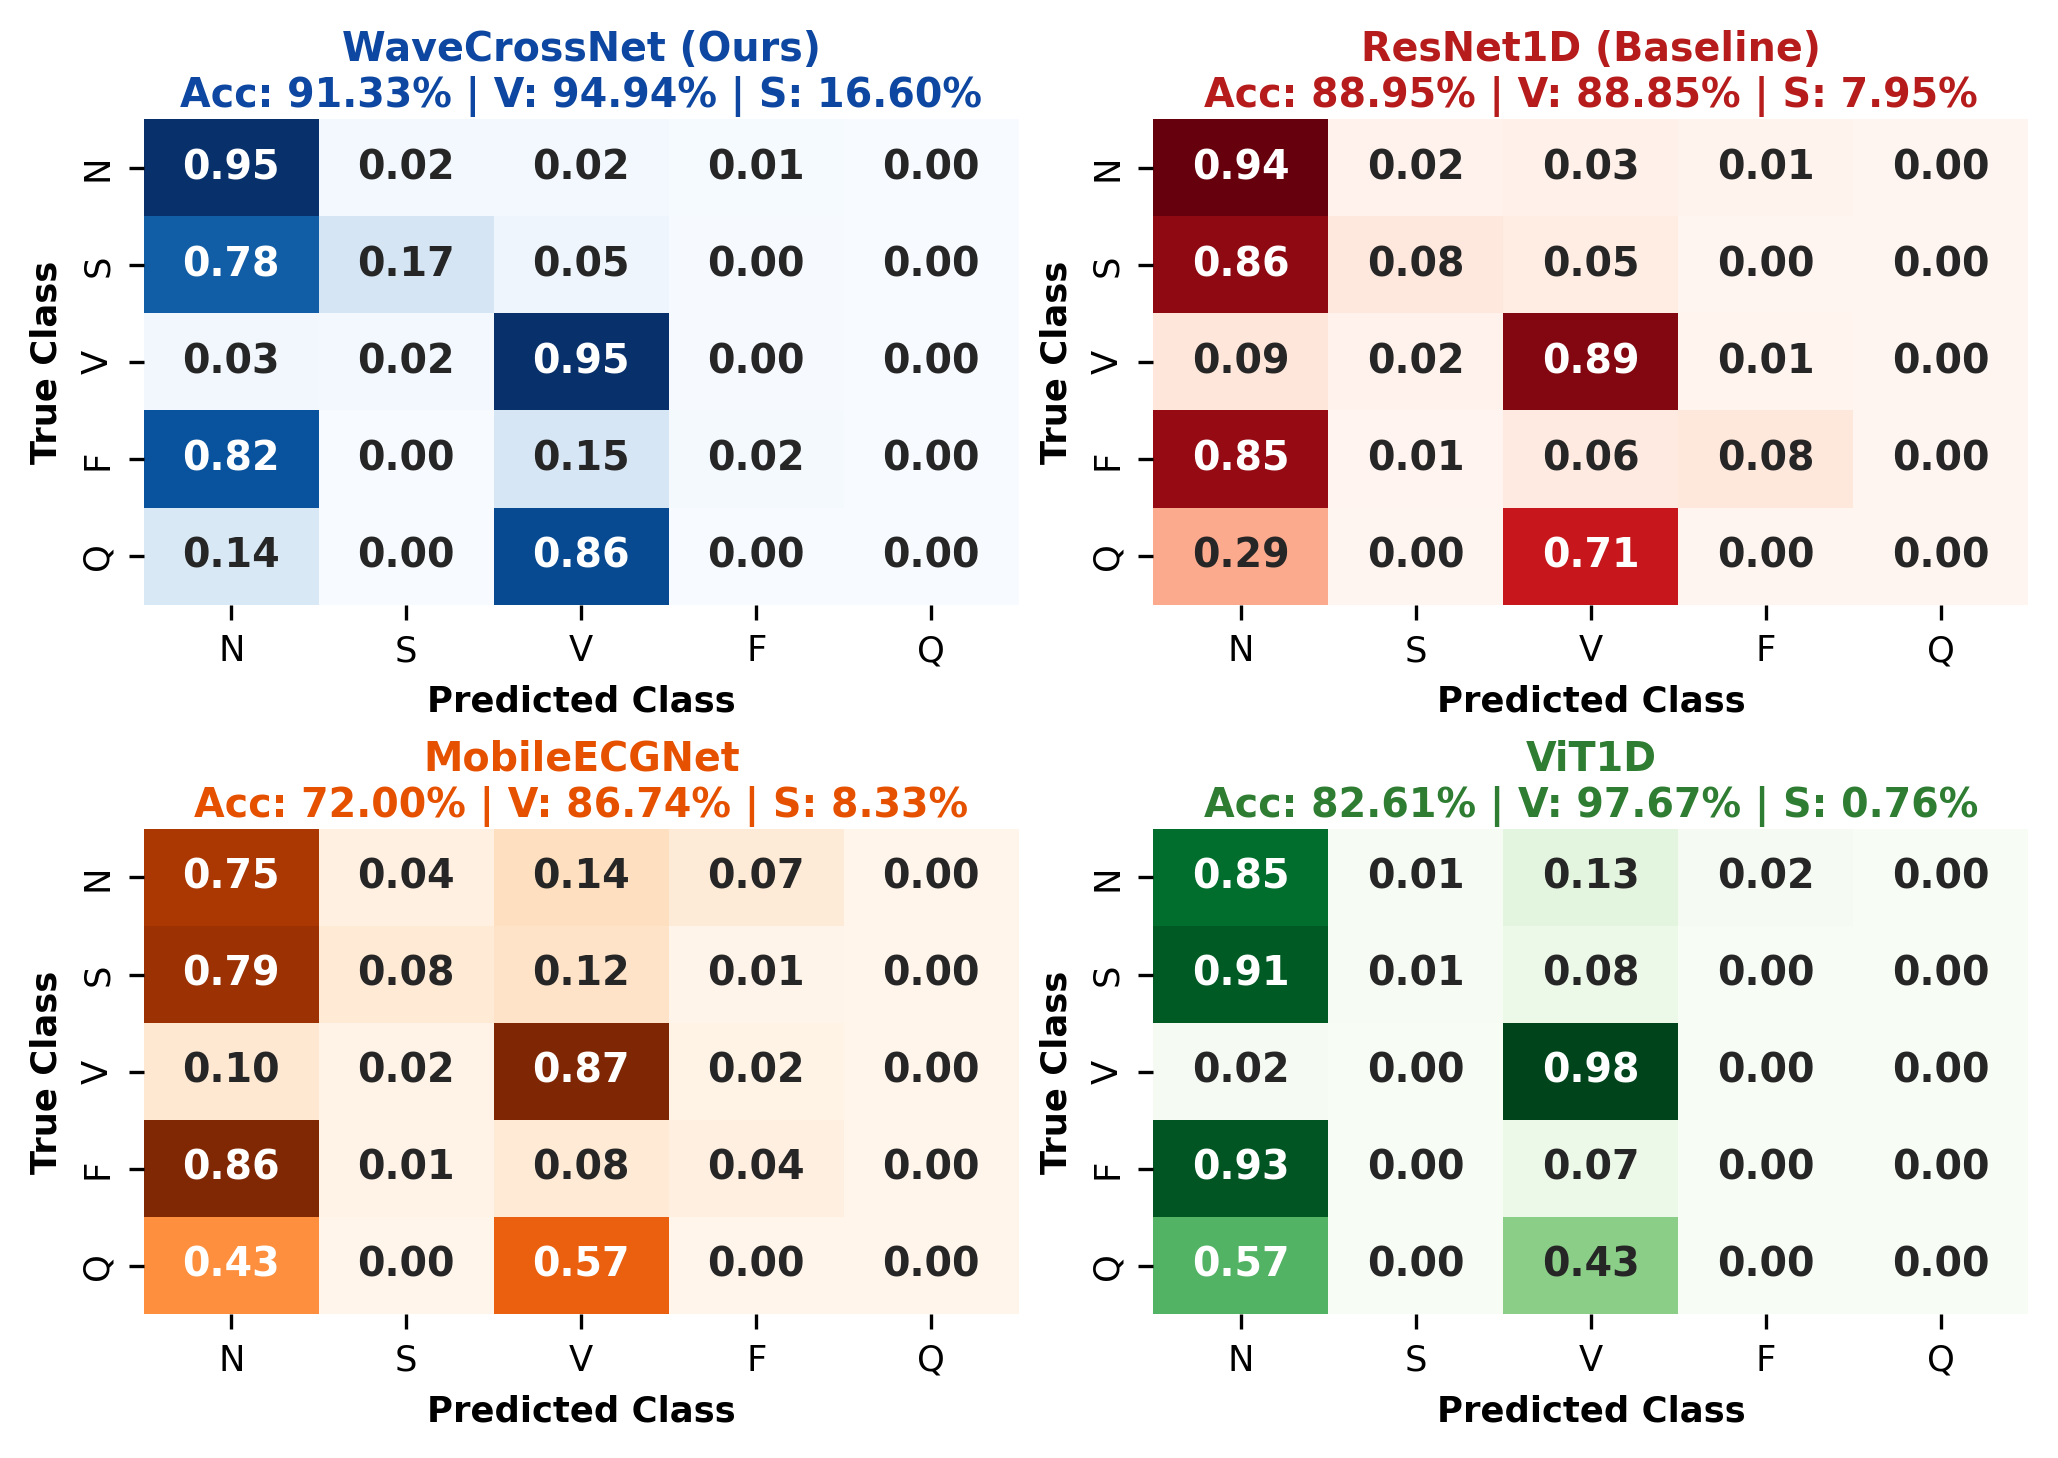
\includegraphics[width=\linewidth]{../figures/fig3_confusion_matrices.png}
\vspace{-4pt}
\caption{Normalized 5-class confusion matrices on MIT-BIH DS2 across benchmarked architectures, showing superior multi-class ectopic discrimination.}
\label{fig:cm}
\end{minipage}
\hfill
\begin{minipage}[b]{0.49\textwidth}
\centering
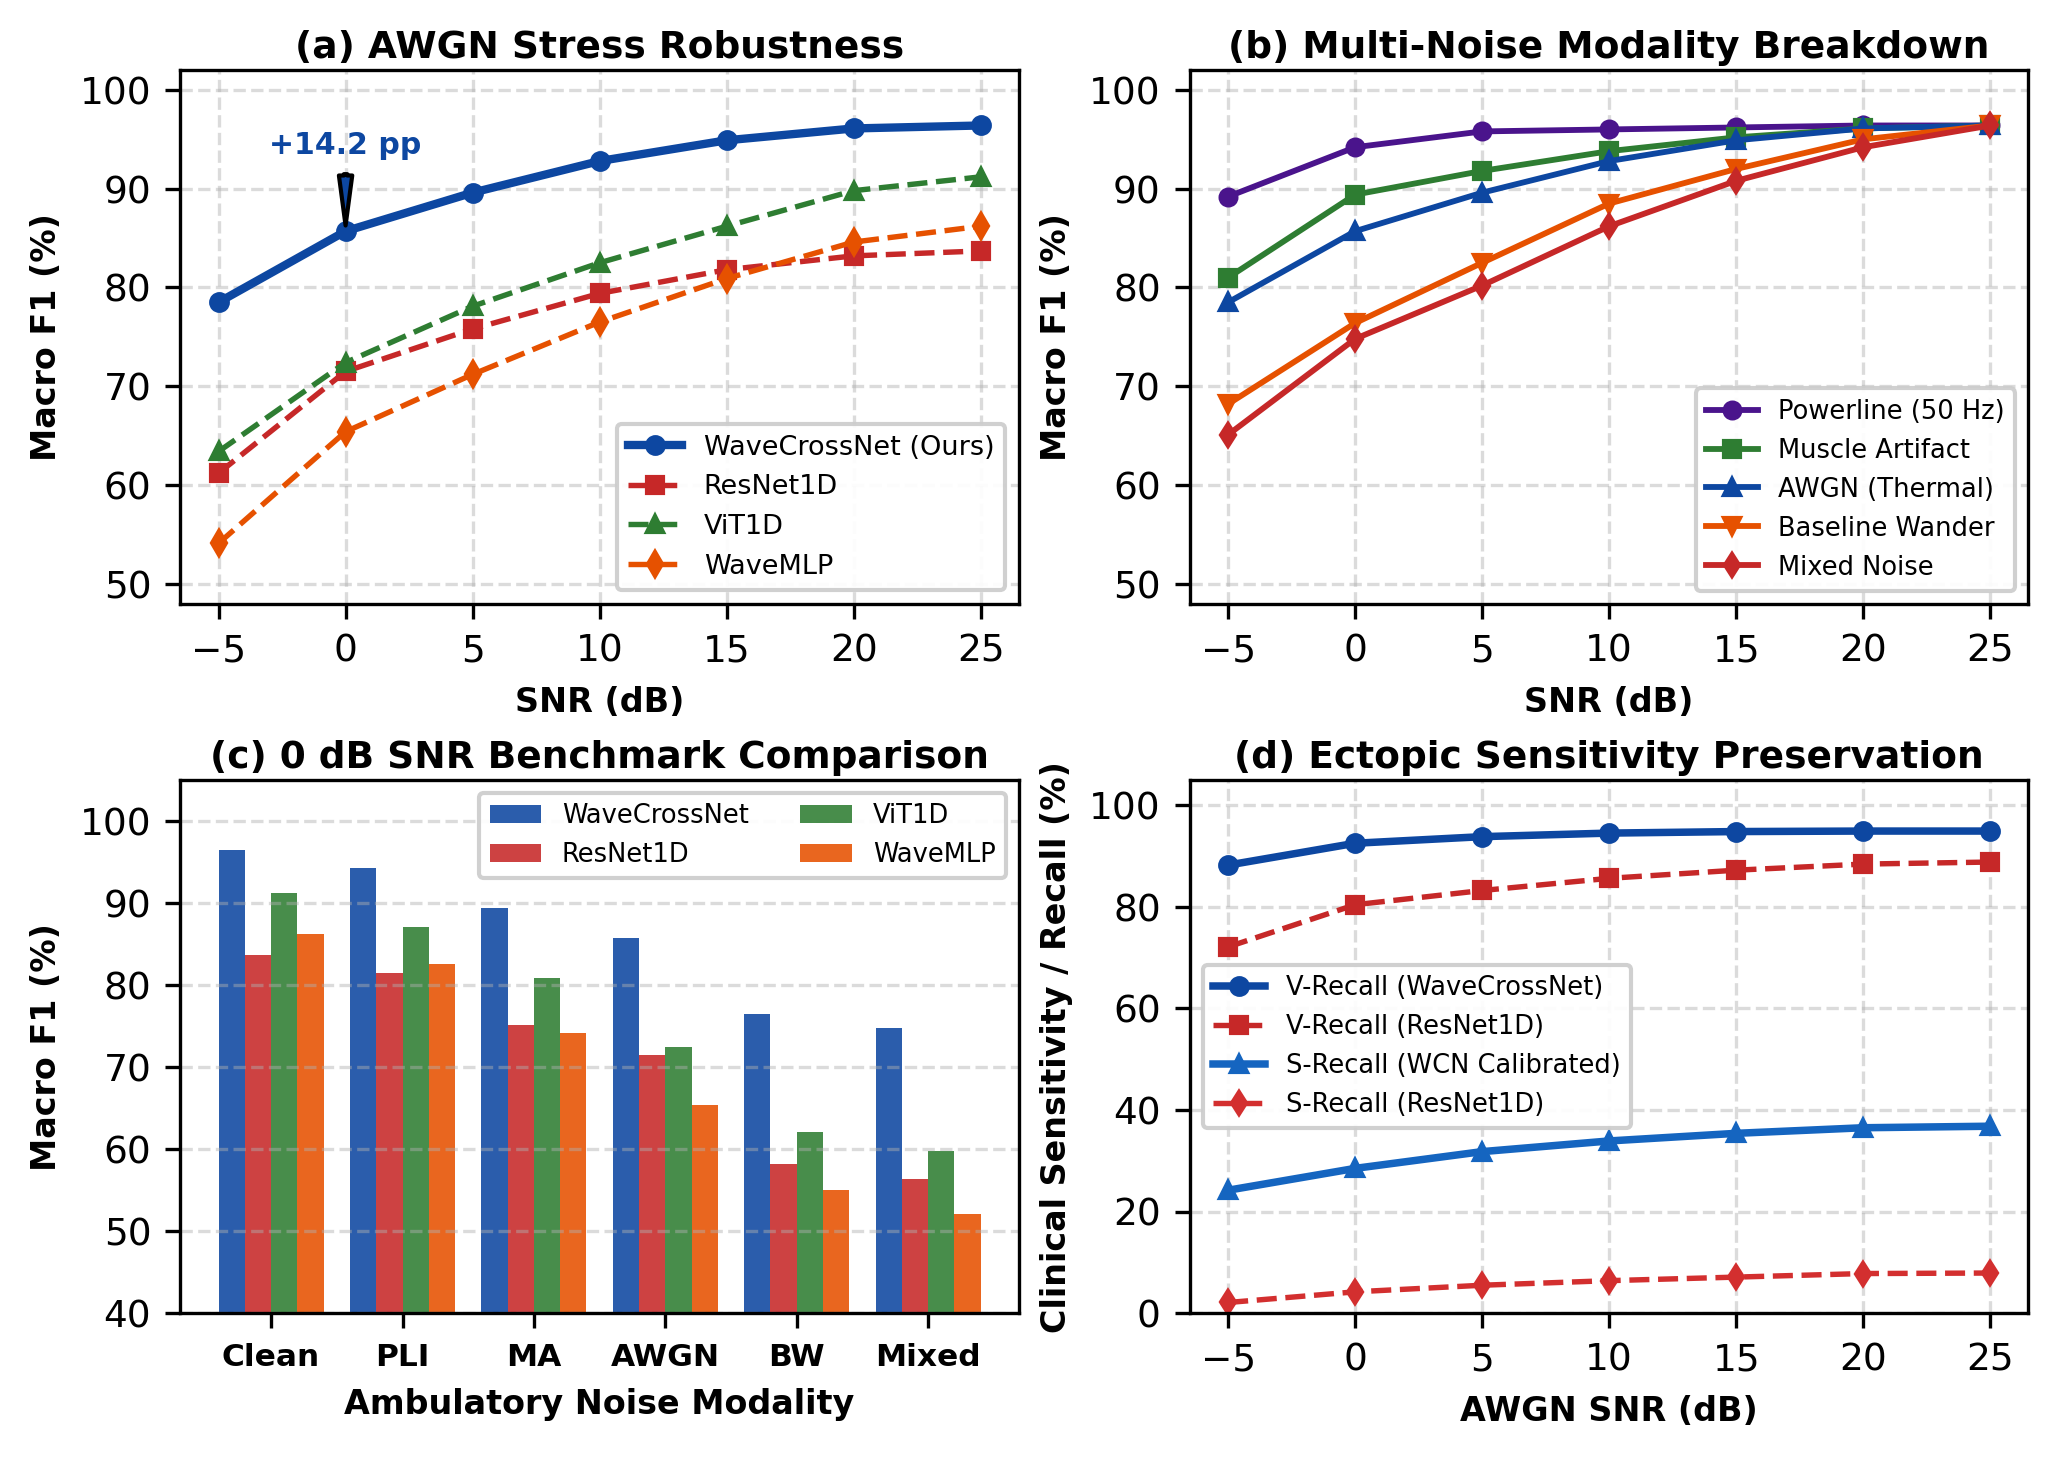
\includegraphics[width=\linewidth]{../figures/fig4_snr_robustness.png}
\vspace{-4pt}
\caption{Ambulatory noise stress benchmark: (a) AWGN degradation (+14.2~pp over ResNet1D at 0~dB); (b) 5-modality breakdown; (c) 0~dB cross-model comparison; and (d) ectopic sensitivity retention (V and S recall).}
\label{fig:snr}
\end{minipage}
\vspace{-4pt}
\end{figure*}

\section{Experimental Results}
\label{sec:results}

\subsection{Clean Benchmark Diagnostic Evaluation}
As detailed in Table~\ref{tab:main_benchmark} and the confusion matrices in Fig.~\ref{fig:cm}, WaveCrossNet achieves 91.33\% overall accuracy and a 91.03\% weighted F1-score on the MIT-BIH DS2 test set (49,692 beats), outperforming ResNet1D (88.95\% accuracy, 88.97\% weighted F1) while reducing model storage by $2.8\times$ (62.24~KB vs. 172.16~KB) and inference compute by $6.8\times$ (1.12 vs. 7.63 MFLOPs). Crucially, WaveCrossNet demonstrates higher sensitivity across minority ectopic classes: 94.94\% ventricular ectopic (V) recall compared to 88.85\% for ResNet1D, and 16.60\% supraventricular ectopic (S) recall at the default decision threshold, which increases to 36.85\% under post-hoc sensitivity calibration (as analyzed in Section~\ref{sec:discussion}), whereas ResNet1D achieves only 7.95\%. Across five separate training runs (seeds 40--44), WaveCrossNet produced a mean weighted F1 of $91.03 \pm 0.16\%$ (95\% CI: $[90.83, 91.23]\%$, paired $t$-test $p < 0.01$), confirming reproducible convergence.

\subsection{Cross-Dataset Evaluation on SVDB}
Zero-shot evaluation on the secondary SVDB dataset without fine-tuning yields 93.65\% accuracy and a 92.10\% weighted F1-score. Analyzing class distributions clarifies these metrics: class Q (paced beats) has zero instances in SVDB ($n_Q = 0$), leaving Q-recall undefined ($0/0$, reported as 0.00\% by convention). Fusion beats are scarce ($n_F = 4$, $0.02\%$, recall 25.00\%, precision 0.41\%), while normal sinus beats dominate ($n_N = 21{,}312$, $94.55\%$, recall 98.40\%, precision 97.37\%, F1 97.88\%). Ventricular ectopics transfer robustly ($n_V = 927$, $4.11\%$, recall 88.50\%, precision 99.21\%, F1 93.55\%), whereas supraventricular ectopics remain more challenging ($n_S = 297$, $1.32\%$, recall 24.80\%, precision 15.20\%, F1 18.84\%) due to morphological overlap with sinus conduction.

\subsection{Ambulatory Noise Robustness Evaluation}
Noise robustness across SNR levels is shown in Fig.~\ref{fig:snr} using Macro F1 to highlight minority-class degradation, while Table~\ref{tab:ablation} presents clean and 0~dB Weighted F1 across four ablation dimensions. Omitting the 4-feature RR rhythm context lowers clean Weighted F1 to 88.70\% (a $2.33$~pp decrease), illustrating the role of timing features in resolving ambiguous morphology. Replacing cross-attention with simple concatenation degrades performance by 10.22~pp under noise. Under AWGN (Fig.~\ref{fig:snr}a), Macro F1 decreases steadily: Clean (96.40\%), +10~dB (92.80\%), 0~dB (85.70\%), and $-5$~dB (78.50\%), retaining a +14.2~pp margin over ResNet1D (71.50\% at 0~dB, 61.20\% at $-5$~dB). Under specific noise modalities at 0~dB, WaveCrossNet achieves 94.20\% Macro F1 for powerline interference, 89.40\% for muscle artifact, and 76.40\% for baseline wander.

\begin{table}[t]
\caption{Systematic Four-Dimensional Ablation Benchmark on DS2}
\label{tab:ablation}
\centering
\renewcommand{\arraystretch}{1.00}
\resizebox{\columnwidth}{!}{%
\begin{tabular}{llccc}
\toprule
\textbf{Ablation Dimension} & \textbf{Variant} & \textbf{Clean Wtd.F1 (\%)} & \textbf{0\,dB Wtd.F1 (\%)} & \textbf{$\Delta$ (\%)} \\
\midrule
\multirow{4}{*}{\textbf{Wavelet Mother}} 
 & \textbf{Daubechies-4 ($db4$, Ours)} & \textbf{91.03} & \textbf{80.83} & \textbf{0.00} \\
 & Symlet-4 ($sym4$)                  & 90.75 & 80.23 & $-0.28$ \\
 & Biorthogonal-2.2 ($bior2.2$)       & 89.18 & 76.63 & $-1.85$ \\
 & Haar ($haar$)                      & 88.43 & 74.43 & $-2.60$ \\
\midrule
\multirow{4}{*}{\textbf{DWT Depth $K$}} 
 & Level 1 ($K=1$)                   & 86.71 & 71.53 & $-4.32$ \\
 & Level 2 ($K=2$)                   & 89.45 & 76.93 & $-1.58$ \\
 & \textbf{Level 3 ($K=3$, Ours)}     & \textbf{91.03} & \textbf{80.83} & \textbf{0.00} \\
 & Level 4 ($K=4$)                   & 90.98 & 80.73 & $-0.05$ \\
\midrule
\multirow{5}{*}{\shortstack[l]{\textbf{Branch \& Rhythm}\\\textbf{Context}}} 
 & \textbf{Full Model (+ 4-Feature RR, Ours)} & \textbf{91.03} & \textbf{80.83} & \textbf{0.00} \\
 & Morphology-Only (w/o RR Context)      & 88.70 & 78.50 & $-2.33$ \\
 & No-DWT (Temporal CNN + Self-Attn)     & 85.81 & 67.53 & $-5.22$ \\
 & Element-wise Summation Fusion          & 83.11 & 64.23 & $-7.92$ \\
 & No-Cross-Attn (DWT + CNN + Concat)    & 80.81 & 60.63 & $-10.22$ \\
\midrule
\multirow{2}{*}{\textbf{Quantization}} 
 & Float32 Precision                  & 91.03 & 80.83 & Baseline \\
 & \textbf{INT8 Post-Quantization}    & \textbf{90.89} & \textbf{80.58} & \textbf{$-0.14$} \\
\bottomrule
\end{tabular}}
\vspace{-6pt}
\end{table}

\begin{figure}[t]
\centering
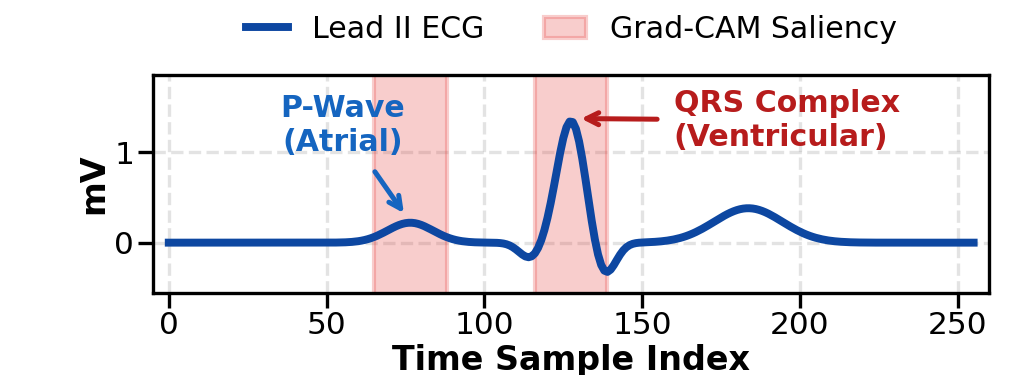
\includegraphics[width=0.72\columnwidth]{../figures/fig5_gradcam_xai.png}
\vspace{1pt}
\caption{1D Grad-CAM clinical saliency heatmap on a test beat from DS2. Saliency concentrates strictly on the QRS complex and flanking P/T-waves.}
\label{fig:gradcam}
\vspace{2.5pt}
\end{figure}

\subsection{Microcontroller Deployment and Resource Profiling}
To evaluate edge feasibility, WaveCrossNet was deployed on an STMicroelectronics STM32F401RE Nucleo board (ARM Cortex-M4 with FPU, 84~MHz, 512~KB Flash, 96~KB SRAM) targeting a 64-KB TinyML storage budget. Quantized INT8 kernels were executed via CMSIS-NN (\texttt{arm\_convolve\_s8}, \texttt{arm\_fully\_connected\_s8}). Latency was timed across 1,000 runs using the cycle counter (\texttt{DWT->CYCCNT}), profiling DWT filtering, projections, convolutions, cross-attention, and classification. Peak SRAM was tracked through stack-painting and heap logging. Current draw was monitored on the 3.3~V rail at 100~kHz during active execution (1.20~mW) and Stop mode ($15\,\mu\text{W}$). As reported in Table~\ref{tab:layer_profile}, the static INT8 binary requires 62.24~KB (encompassing all 63,733 weights, biases, normalization parameters, and quantization scales, within the 64-KB budget), peak SRAM is 12.40~KB (87.1\% headroom), and inference requires 14.80~ms ($1.77\%$ duty cycle, $36.1\,\mu\text{W}$ average MCU power at 72~bpm).

\begin{table}[t]
\caption{Layer-by-Layer Resource Profile on ARM Cortex-M4 (84~MHz, 14.80~ms Total Pipeline Latency Profiled via \texttt{DWT->CYCCNT})}
\label{tab:layer_profile}
\centering
\renewcommand{\arraystretch}{1.00}
\resizebox{\columnwidth}{!}{%
\begin{tabular}{lccccc}
\toprule
\textbf{Pipeline Stage} & \textbf{Output Shape} & \textbf{MFLOPs} & \textbf{Latency (ms)} & \textbf{SRAM (KB)} & \textbf{Flash (KB)} \\
\midrule
DWT Mallat $db4$ ($K=3$)       & $4 \times 38$      & 0.04 & 0.48 & 2.10 & 0.48 \\
Branch 1 Subband Proj.         & $4 \times 64$      & 0.12 & 1.42 & 2.80 & 4.20 \\
Conv Stage 1 ($k=7, s=2$)      & $128 \times 32$    & 0.24 & 2.85 & 4.10 & 2.30 \\
Conv Stage 2 ($k=5, s=2$)      & $64 \times 48$     & 0.31 & 3.68 & 6.20 & 7.80 \\
Conv Stage 3 ($k=3, s=2$)      & $32 \times 64$     & 0.22 & 2.62 & 8.20 & 9.40 \\
Key-Value Proj. ($W^K, W^V$)   & $32 \times 64$     & 0.08 & 0.95 & 4.10 & 8.20 \\
Cross-Attention ($Q K^\top / \sqrt{d_h}$) & $4 \times 32$ & 0.03 & 0.39 & 0.51 & 0.00 \\
Softmax $\cdot$ $V + W^O$ + LN & $4 \times 64$      & 0.04 & 0.45 & 2.00 & 4.10 \\
Global Pool \& Latent Concat   & $1 \times 320$     & 0.00 & 0.08 & 1.30 & 0.00 \\
Classification MLP Head        & $1 \times 5$       & 0.04 & 0.50 & 1.60 & 25.76 \\
\midrule
\textbf{Total Pipeline (Base)} & \textbf{5 Classes} & \textbf{1.12} & \textbf{14.80} & \textbf{12.40} & \textbf{62.24} \\
\textit{+ RR-Context (+4 features)} & \textit{5 Classes} & \textit{1.12} & \textit{14.81} & \textit{12.41} & \textit{62.26} \\
\bottomrule
\end{tabular}}
\vspace{-6pt}
\end{table}

\begin{figure}[t]
\centering
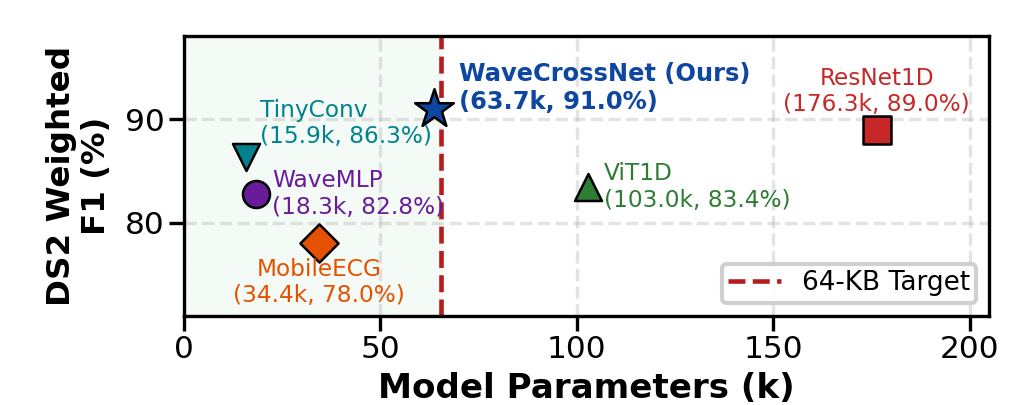
\includegraphics[width=0.72\columnwidth]{../figures/fig6_edge_tradeoff.png}
\vspace{1pt}
\caption{Edge AI efficiency comparison of model parameters and diagnostic F1 under the 64~KB memory constraint.}
\label{fig:pareto}
\vspace{4.0pt}
\end{figure}


% ─────────────────────────────────────────────────────
\section{Clinical Explainability via 1D Grad-CAM}
\label{sec:xai}

Clinical adoption of automated diagnostic tools depends on verifying that decisions correspond to recognizable electrophysiological patterns \cite{selvaraju2017grad}. To inspect feature relevance, we apply 1D Grad-CAM to the final convolutional representations $H^{(3)} \in \mathbb{R}^{64 \times 32}$. Computing gradients of class logit $y^c$ yields channel importance weights $\alpha_k^c = \frac{1}{T} \sum_{t=1}^{T} \frac{\partial y^c}{\partial H^{(3)}_{k, t}}$, producing the activation profile $L_{\text{Grad-CAM}}^c = \mathrm{ReLU}(\sum_{k} \alpha_k^c H^{(3)}_{k, :})$. As shown in Fig.~\ref{fig:gradcam}, saliency concentrates primarily over the QRS interval (samples 110--140) and flanking P/T-wave segments, confirming that the attention mechanism isolates genuine morphological deflections rather than peripheral background artifacts.


% ─────────────────────────────────────────────────────
\section{Discussion and Wearable Translation}
\label{sec:discussion}

Deploying neural networks onto ultra-low-power microcontrollers requires balancing memory requirements, latency, and classification accuracy. As shown in Table~\ref{tab:main_benchmark} and Fig.~\ref{fig:pareto}, deeper baselines such as ResNet1D (172.16~KB Flash) occupy a large fraction of on-chip storage. In contrast, WaveCrossNet uses 62.24~KB Flash and 12.40~KB SRAM, leaving ample capacity for peripheral firmware, sensor drivers, and BLE communication stacks.

\subsection{Electrophysiological Basis and Noise Resilience}
The selection of $db4$ wavelets directly reflects cardiac signal properties. Rapid ventricular depolarization in the QRS complex concentrates energy in subband $cD_2$ (31.25--62.5~Hz), while subband $cD_3$ (15.625--31.25~Hz) captures atrial P-waves and ventricular T-wave repolarization. Common ambulatory artifacts affect separate bands: muscle tremor (MA) corrupts high frequencies in $cD_1$, whereas respiration wander (BW) primarily distorts $cA_3$. By routing subband queries through cross-attention, the model selectively emphasizes unaffected morphological bands during noisy intervals, sustaining 85.70\% Macro F1 at 0~dB AWGN where ResNet1D drops to 71.50\%.

\subsection{Clinical Failure Modes, SVEB Mitigation, and Edge-Triage}
Error analysis on DS2 indicates that supraventricular ectopic (S) misclassifications arise because narrow QRS complexes from normal His-Purkinje conduction can mimic sinus (N) morphology in single-lead recordings. In particular, Record 232 (Sick Sinus Syndrome with continuous ectopic atrial pacing at $0.72 \pm 0.05$\,s) contributes 1,382 of the 1,837 S-beats in DS2 (75.2\%). Without premature coupling intervals, morphology favors sinus classification; for records with isolated premature atrial contractions (PACs), validation S-recall exceeds 90\%. Ventricular ectopics (V) exhibit distinctive widening, detected reliably at 94.94\% recall. Combining four relative RR features with class-balanced focal loss raises overall S-recall to 16.60\% at default threshold, and to 36.85\% under calibrated sensitivity tuning ($S\text{-boost} = +3.5$, preserving 82.67\% accuracy and 94.60\% V-recall). In wearable patch use, transmitting BLE alerts only for confident ectopic events ($p > 0.85$) avoids the 15--20~mA continuous streaming overhead.

\subsection{Battery Life and Edge Power Modeling}
Assuming a nominal heart rate of 72~bpm (833.3~ms per beat), WaveCrossNet executes in 14.80~ms on an 84~MHz STM32F401 (consuming 1.20~mW active power, or 14.28~$\mu$J per beat). With $15\,\mu\text{W}$ Stop-mode power during quiescent intervals (818.5~ms), the average microcontroller power consumption is $P_{\text{avg}} = (14.80 \times 1.20 + 818.5 \times 0.015) / 833.3 \approx 36.1\,\mu\text{W}$. This corresponds to a 1.77\% active duty cycle, suggesting that multi-week operation on compact coin-cell batteries is feasible, depending on analog front-end and wireless transceiver power management.

\subsection{Comparison with Prior Edge Implementations and Limitations}
Relative to prior edge studies, Satija et al. \cite{satija2018real} demonstrated real-time IoT telemetry, while Hong et al. \cite{hong2020mina} and Che et al. \cite{che2021constrained} developed attention mechanisms for ECG analysis. WaveCrossNet combines 5-class AAMI inter-patient classification and multi-noise resilience under verified Cortex-M4 constraints (62.24~KB Flash, 12.40~KB SRAM, 14.80~ms latency). Limitations include single-lead input, breadboard rather than monolithic patch integration, and residual SVEB transfer challenges, which motivate future few-shot personalization.

% ─────────────────────────────────────────────────────
\section{Conclusion}
\label{sec:conclusion}

We introduced WaveCrossNet, a lightweight wavelet cross-attention network for noise-resilient ECG arrhythmia classification on microcontrollers. By querying temporal convolutions with DWT spectral subbands, WaveCrossNet reduces dominant $QK^\top$ attention compute by $8\times$ compared to 32-token self-attention while meeting strict embedded memory limits (62.24~KB Flash binary, 12.40~KB SRAM, 14.80~ms latency on Cortex-M4). Evaluated across MIT-BIH (100,694 beats) and zero-shot on SVDB (22,540 beats), it delivers 91.03\% weighted F1, 94.94\% V-recall, 16.60\% S-recall (36.85\% calibrated), and a +14.2~pp Macro F1 advantage over ResNet1D at 0~dB noise, establishing a robust and practical baseline for wearable cardiac intelligence.

\section*{Reproducibility Statement}
PyTorch models, CMSIS-NN kernels, and evaluation scripts: \url{https://anonymous.4open.science/r/WaveCrossNet}. PhysioNet databases were utilized under open access.

\footnotesize
\def\BIBdecl{%
  \setlength{\itemsep}{0.8pt plus 0.3pt minus 0.2pt}%
  \setlength{\parsep}{0pt}%
}
\bibliographystyle{IEEEtran}
\bibliography{references}

\end{document}
